\documentclass[12pt, a4paper, oneside]{amsart}
\setlength{\parindent}{0pt}
\usepackage[margin=2cm]{geometry}
\usepackage{amsmath}
\usepackage{amssymb}
\usepackage{amsfonts}
\usepackage[pdftex]{graphicx}
\usepackage[usenames]{color}
\usepackage{graphicx}
\usepackage{hyperref}
\usepackage{amsthm}

\title{Project 5: Text Manipulation on E-Mail Messages}
\author{Kevin Fujii and Erin Melcon}
\date{\today}

\begin{document}

\maketitle

\section*{Project Overview}

In this assignment, we focus on manipulating text data into a desirable form and analyzing the structured data through the application of regular expressions.  We will be using two large data sets for this project.  The first data set is composed of all e-mails from Enron before the company folded.  The second contains the archive of the R-help mailing list from April 1998 to February 2011.  The data sets have several aspects in common, so we can use these characteristics to create general functions that should be compatible with all e-mail files.

\section*{R-Help mailing list}

\subsection{Format of the data}

The R-help mailing list archive is stored as 167 .tar.gz files corresponding to each month from April 1998 to February 2011.  Each of the .tar.gz files is a compressed text file consisting of all e-mail messages send through the mailing list during that month.  E-mail volume per month varies from 36 to 8674 messages, and there is an increasing trend through time.  A plot of the e-mail messages sent per month may be seen in Figure \ref{fig:rhelpByMonth}.

\begin{figure}[htp]
\centering
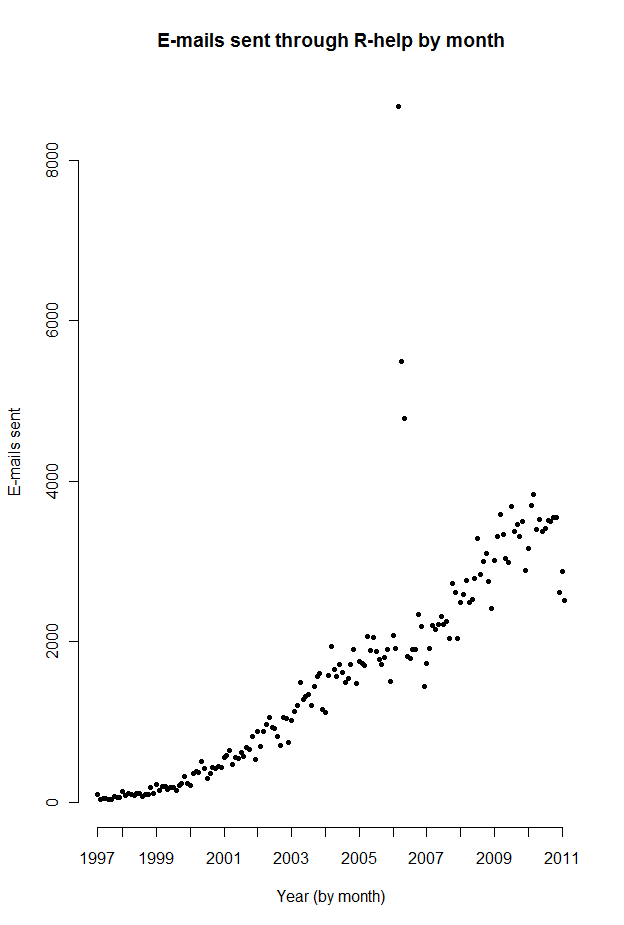
\includegraphics[width = 100mm]{rhelpByMonth.png}
\caption{From 1998 to 2011, the popularity of the R-help mailing list appears to grow exponentially with some unexpectedly high traffic during 2006.}\label{fig:rhelpByMonth}
\end{figure}

Upon closer inspection, the spike in e-mail volume seen in Figure \ref{fig:rhelpByMonth} occurs in March 2006.  As a diagnostic check, we can look at the file size corresponding to the compressed file of that month's e-mail messages, and sure enough, the March 2006 file is much larger than the other files.  We can take a closer look at e-mail volume by inspecting the data set by day rather than by month.  A histogram of e-mail volume by day is shown in Figure \ref{fig:rhelpByDay}.

\begin{figure}[htp]
\centering
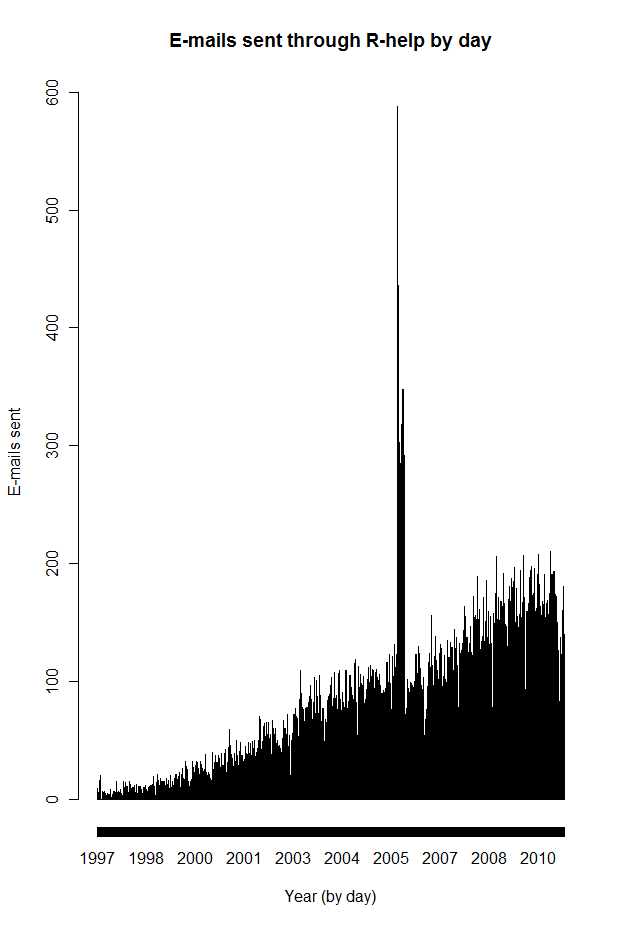
\includegraphics[width = 100mm]{rhelpByDay.png}
\caption{The e-mail volume appears to grow when we look at e-mails sent per day.  The peaks occur in March 2006, when around 500 e-mails were sent on multiple days.}\label{fig:rhelpByDay}
\end{figure}

Somewhat unsurprisingly at this point, the 49 days with the most e-mails sent through the R-help mailing list all occurred in 2006.  All of these 49 days fell in March, April, or May of that year.  

\subsection{Functions of interest}

We can use regular expressions in order to search the subjects and bodies of the R-help e-mails for function calls.  First, let's look through the subject lines.  A search with regular expressions found 19150 possible uses of functions in subject lines, the most common of which are tabulated in the first two columns of Table \ref{table:allFcns}.

 \begin{table}[ht]
 \centering
 \begin{tabular}{|c|c||c|c|}
 \hline
\multicolumn{2}{|c||}{Subject Line} & \multicolumn{2}{|c|}{E-Mail Body}\\
\hline
\footnotesize{\textbf{Function}}& \footnotesize{\textbf{Frequency}} & \footnotesize{\textbf{Function}}& \footnotesize{\textbf{Frequency}}\\
\hline
lm & 527 & c & 169356 \\
plot & 465 & function & 55049\\
par & 326 & list & 39738\\
library & 242 & library & 31071\\
apply & 213 & plot & 30538\\
optim & 194 & length & 29409\\
glm & 191 & rep & 28783\\
source & 191 & rnorm & 24379\\
c & 183 & data.frame & 22974\\
summary & 181 & paste & 21357\\
lme & 178 & matrix & 20023\\
image & 166 & lm & 16186\\
\hline
\end{tabular}
\caption{The twelve most commonly referenced functions in subject lines and e-mail bodies from the R-help mailing list.}
\label{table:allFcns}
\end{table}

The functions appearing in Table \ref{table:allFcns} are all quite common, as expected.  Several of them (also including \textit{lmer}, not listed in Table \ref{table:allFcns}) refer to various types of linear models, indicating that many people are using the R-help mailing list for advice or troubleshooting when performing data analysis.  Further, graphical and summarizing functions appear on the list, which are used to visually or numerically summarize a data set.

Now, let's look at the functions used in the bodies of the e-mail messages.  The most commonly used functions in e-mail bodies are displayed in the third and fourth columns of Table \ref{table:allFcns}.  It should come as no surprise that the functions used in e-mail bodies are even more generic than those in subject lines.  Users of the R-help mailing list are likely to include their code in the bodies of their e-mails, so it makes sense that these generic functions appear most often since they have wide applications.  Many of these functions deal with data creation, possibly to set up test data for more complex function calls.

We can also explore what packages the users of the R-help mailing list are utilizing.  The most commonly loaded packages are shown in Table \ref{table:allLibs}.

 \begin{table}[ht]
 \centering
 \begin{tabular}{|c|c||c|c|}
 \hline
\multicolumn{2}{|c||}{Subject Line} & \multicolumn{2}{|c|}{E-Mail Body}\\
\hline
\footnotesize{\textbf{Library}}& \footnotesize{\textbf{Frequency}} & \footnotesize{\textbf{Library}}& \footnotesize{\textbf{Frequency}}\\
\hline
survival & 13 & lattice & 2392 \\
car &10 & zoo & 1384\\
MASS & 10 & MASS & 1345\\
gplots & 9 & nlme & 1005\\
Matrix & 9 & ggplot2 & 824\\
... & 8 & Hmisc & 604\\
tcltk & 8 & chron & 555\\
fCalendar & 6 & lme4 & 497\\
SSPA & 6 & tcltk & 477\\
``package'' & 5 & RODBC & 471\\
svIDE & 5 & gsubfn & 393\\
convert & 4 & survival & 375\\
\hline
\end{tabular}
\caption{The twelve most commonly referenced libraries in subject lines and e-mail bodies from the R-help mailing list.}
\label{table:allLibs}
\end{table} 





\newpage
\section{Enron Email List}
The main purpose of this part of the project is to find all the email recipients and senders from the Enron data set, and summarize and graphically represent the results.  The first task was to extract the header of the emails, and from this extract all of the information about who sent the email, and who it was sent to.  This included looking for Bcc (Blind Carbon Copy) and Cc (Carbon Copy) fields.\\
This was accomplished using regular expressions, and we found that if we do not include Bcc and Cc, we see that the person who emailed anyone the most was Jeff Dasovich.  If we include Bcc and Ccs, the list remains the same.  We may now want to investigate who Jeff was emailing, and we have two ways of doing that.\\ 
\begin{table}[h]
\begin{center}
\begin{tabular}{|r|l|r|}
  \hline
Rank & Sender & Number of Emails \\ 
  \hline
1 & jeff.dasovich@enron.com & 131302 \\ 
2 & veronica.espinoza@enron.com & 110601 \\ 
3 & rhonda.denton@enron.com & 90730 \\ 
4 & cheryl.johnson@enron.com & 74632 \\ 
5 & jae.black@enron.com & 59196 \\ 
 \hline
\end{tabular}
\caption{The top 5 people who sent email from the Enron email list.}
\label{table:allLibs}
\end{center}
\end{table}

The first is to build another frequency table, as follows:
\begin{table}[h]
\begin{center}
\begin{tabular}{|r|l|l|l|}
  \hline
Rank & Sender & Recipient & Frequency \\ 
  \hline
 1 & jeff.dasovich@enron.com & richard.shapiro@enron.com & 2909 \\ 
  2 & jeff.dasovich@enron.com & paul.kaufman@enron.com & 2768 \\ 
  3 & jeff.dasovich@enron.com & susan.mara@enron.com & 2746 \\ 
  4 & jeff.dasovich@enron.com & james.steffes@enron.com & 2725 \\ 
  5 & jeff.dasovich@enron.com & karen.denne@enron.com & 2489 \\ 
   \hline
\end{tabular}
\caption{The top five people that Jeff Dasovich emailed.}
\label{table:allLibs}
\end{center}
\end{table}
In which we can see the number of times Jeff emailed his top 5 recipients.  We may also look at a network graph;
\begin{figure}[htp]
\centering
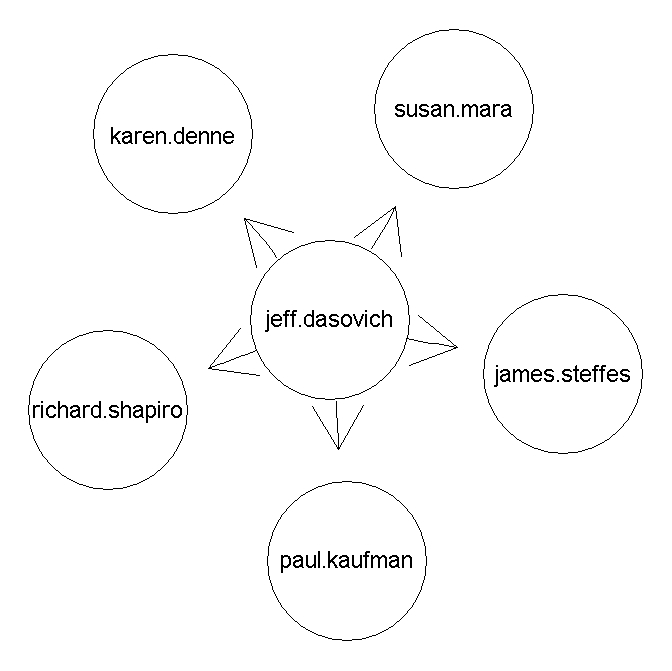
\includegraphics[width = 100mm]{JeffPlot.jpeg}
\caption{A small network of who Jeff emails}\label{fig:JeffNetwork}
\end{figure}\\
Which gives us the same information, but visually, and without information about the weights.  However, with network graphs it is easy to see who people Jeff emailed were communicating with.  
\begin{figure}[htp]
\centering
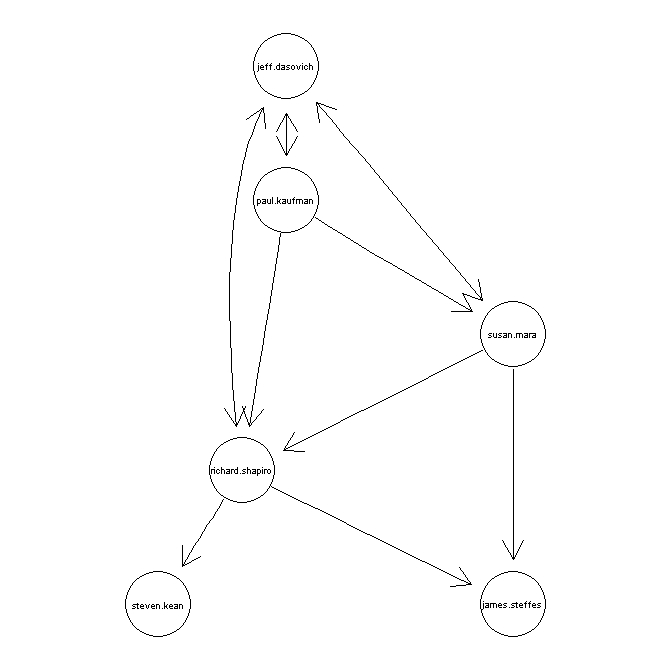
\includegraphics[width = 100mm]{JeffPlot2.jpeg}
\caption{A small network of who Jeff emails, and who they email.}\label{fig:JeffNetwork}
\end{figure}\\


\end{document}